%%%%%%%%%%%%%%%%%%%%%%%%%%%%%%%%%%%%%%%%%%%%%%%%%%%%%%%%%%%%%%%%%%%%%%%%%%%%%%%
%% 2.- QUE ES UNA UTA
%%%%%%%%%%%%%%%%%%%%%%%%%%%%%%%%%%%%%%%%%%%%%%%%%%%%%%%%%%%%%%%%%%%%%%%%%%%%%%%

\cleardoublepage
\chapter{Las Unidades de Tratamiento de Aire}
\chaptermark{Las Unidades de Tratamiento de Aire}

\label{chap:anexoUTA} % etiqueta para poder referenciar luego en el texto con ~\ref{sec:intro}
% \addcontentsline{toc}{chapter}{Introducción, Objetivos, Metodología y Planificación

Una UTA es un equipo encargado de tratar el aire atendiendo a distintos aspectos de la climatización:

\begin{itemize}
    \item Ventilación
    \item Filtrado
    \item Control de temperatura
    \item Control de humedad
\end{itemize}

Su funcionamiento da la posibilidad de regular el caudal de ventilación en función de la medición del CO2 y de las condiciones térmicas del local, así como recuperar parte de la energía térmica del aire que se expulsa al exterior.

Las partes de las que se compone una UTA son:

\begin{itemize}
    \item Compuertas o tomas para la entrada y salida de aire.
    \item Zona de mezcla del aire de retorno y del aire exterior para permitir recuperar energía mediante lo que se conoce como \textit{free-cooling}. La recuperación puede ser de distintos tipos:
    \begin{itemize}
        \item Recuperación aire-agua: el aire extraído transfiere su calor al agua a través de un intercambiador. El mismo agua transfiere ese calor al aire introducido desde el exterior, el cual fluye por otro conducto. Este sistema es más salubre al impedir que se mezclen ambas corrientes de aire, pero tiene menor rendimiento.
        \item Recuperación mediante placas aire-aire: a través de un cubo metálico pasan ambas corrientes de aire a modo de flujo cruzado. El calor se transfiere a través del contacto del aire con las placas metálicas de los canales.
    \end{itemize}
    \item Intercambiador de calor, por donde fluye agua a la temperatura deseada (frío o calor). La temperatura del agua se transfiere al aire cuando éste pasa a través del intercambiador.
    \item Filtros, que pueden ser de distintos tipos en función de las especificaciones de filtrado.
    \item Humectador: el paso del aire seco y caliente por un panel mojado hace que se evapore parte de su agua y se produzca aire húmedo y frío. Dispone de una bandeja de almacenamiento y recogida del agua.
    \item Zona de ventilación, con ventilador y motor.
\end{itemize}

La siguiente figura ilustra a modo de ejemplo todos los elementos mencionados:

\begin{figure}[H]
    \centering
    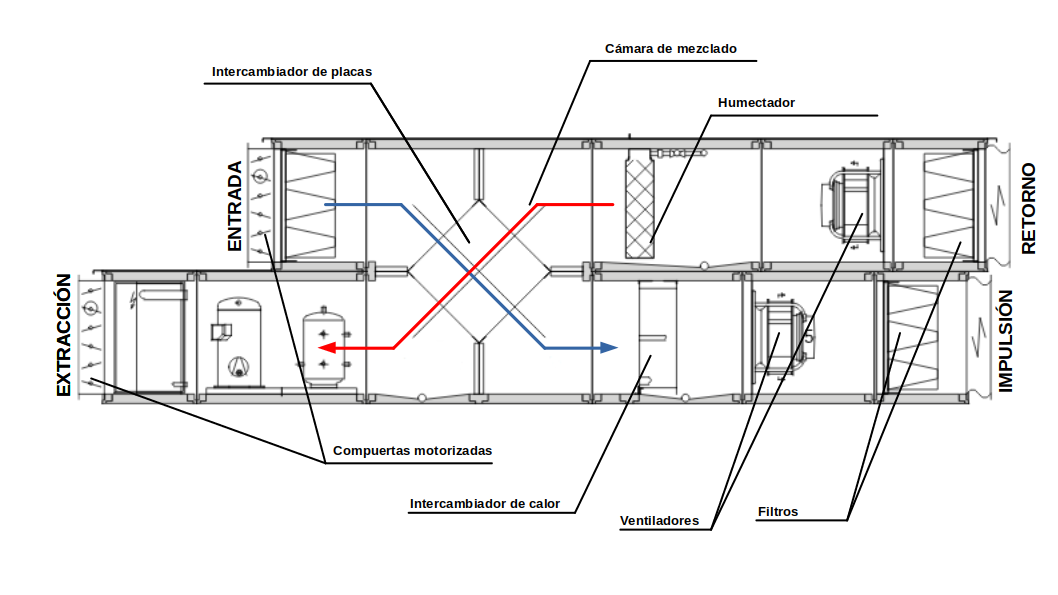
\includegraphics[width=\textwidth, keepaspectratio]{img/esquemaUTA}
    \caption{Plano de partes de una UTA}
    \label{figura:esquemaUTA}
\end{figure}
